%------------------------------------------------------------------%
% Cannabis Data Science Presentation
% Date: 11/10/2021
% Authors: Keegan Skeate <keegan@cannlytics.com>
% Copyright (c) Cannlytics
%------------------------------------------------------------------%
\documentclass[xcolor={dvipsnames}]{beamer}
\hypersetup{pdfpagemode=FullScreen}
\mode<presentation> %TEMPLATE
{ \usetheme{Boadilla}
  \usecolortheme{orchid}
  \usefonttheme{default}
  \setbeamertemplate{navigation symbols}{}
  \setbeamertemplate{caption}[numbered]} 
\usepackage[english]{babel}
\usepackage[utf8x]{inputenc}
\setbeamersize{text margin left=0.5in,text margin right=0.5in}

\usepackage[dvipsnames]{xcolor}
\definecolor{DarkGreen}{RGB}{2, 48, 32}
\definecolor{CalyxGreen}{RGB}{34, 153, 84}
\definecolor{DarkOrange}{RGB}{199, 0, 57}
\definecolor{LightOrange}{RGB}{255, 87, 51}
\definecolor{LightGreen}{RGB}{218, 247, 166}
\definecolor{LightYellow}{RGB}{255, 195, 0}

\setbeamercolor*{palette primary}{bg=LightGreen, fg = DarkGreen}
\setbeamercolor*{palette secondary}{bg=LightGreen, fg=DarkGreen}
\setbeamercolor*{palette tertiary}{bg=LightGreen, fg = DarkGreen}
%\setbeamercolor*{palette quaternary}{bg=myNewColorD, fg = green}

% Margins
%\addtobeamertemplate{frametitle}{}{\vspace{-1em}}
%\setbeamersize{text margin right=5cm}

%------------------------------------------------------------------%
% FIXME: Bibliography
% https://tex.stackexchange.com/questions/148893/package-biblatex-error-incompatible-package-ucs-begindocument?noredirect=1&lq=1
% https://tex.stackexchange.com/questions/261595/how-to-rerun-biber-on-the-file
% https://tex.stackexchange.com/questions/229638/package-biblatex-warning-babel-polyglossia-detected-but-csquotes-missing
% https://tex.stackexchange.com/questions/49610/use-biblatex-and-utf8
% https://stackoverflow.com/questions/1507672/putting-citation-text-on-same-slide-with-latex-beamer
%------------------------------------------------------------------%
%\usepackage{csquotes}
%\usepackage[style=verbose]{biblatex}
%\addbibressource{presentation-bib.bib}

%------------------------------------------------------------------%
% Packages
%------------------------------------------------------------------%
\usepackage{amsmath}
\renewcommand*\footnoterule{} %No sperating line on footnote
\usepackage{mathtools} %ANNOTATING EQUATIONS
\usepackage{hhline} %DOUBLBARS
\newcommand\T{\rule{0pt}{2.5ex}} %TOPSTRUT
\newcommand\B{\rule[-1.25ex]{0pt}{0pt}} %BOTTOMSTRUT
\newenvironment<>{varblock}[2][.9\textwidth] %RESIZED BLOCKS
  {\setlength{\textwidth}{#1}
  \begin{actionenv}#3
    \def\insertblocktitle{#2}\par
    \usebeamertemplate{block begin}}
  {\par\usebeamertemplate{block end}
  \end{actionenv}}
\defbeamertemplate{enumerate item}{largeball} %LARGE BALLS
{\begin{pgfpicture}{-1ex}{-0.65ex}{1.5ex}{1.5ex}
\usebeamercolor[fg]{item projected}
{\pgftransformscale{2.5}\pgftext{\Large\pgfuseshading{bigsphere}}}
{\pgftransformshift{\pgfpoint{0pt}{0.5pt}}
\pgftext{\usebeamerfont*{item projected}\small\insertenumlabel}}
\end{pgfpicture}}
\usepackage{tikz} % FANCY ARROWS
\usepackage{xparse}
\NewDocumentCommand\UpArrow{O{2.0ex} O{black}}{%
   \mathrel{\tikz[baseline] \draw [->, line width=0.5pt, #2] (0,0) -- ++(0,#1);}} % FANCY UPARROW
\NewDocumentCommand\DownArrow{O{2.0ex} O{black}}{%
   \mathrel{\tikz[baseline] \draw [<-, line width=0.5pt, #2] (0,0) -- ++(0,#1);}} % FANCY DOWNARROW
%\vskip 1cm
\makeatletter
\newcommand{\LeftEqNo}{\let\veqno\@@leqno}%LEFT EQUATION #'s
\makeatother

%------------------------------------------------------------------%
% Title
%------------------------------------------------------------------%
\title[Meetup]{}
\author{Cannabis Data Science}
\institute[]{\Large Meetup}
\date{November 10, 2021}
\begin{document}
\begin{frame}{}
  
\includegraphics[scale=0.075]{images/logos/cannlytics_logo_with_text_light.png}
  \titlepage
\end{frame}

%------------------------------------------------------------------%
% Introduction
%------------------------------------------------------------------%

\section{Introduction}

\begin{frame}{}

{\large Predicting Market Performance}\vspace{\baselineskip}\\

\begin{center}
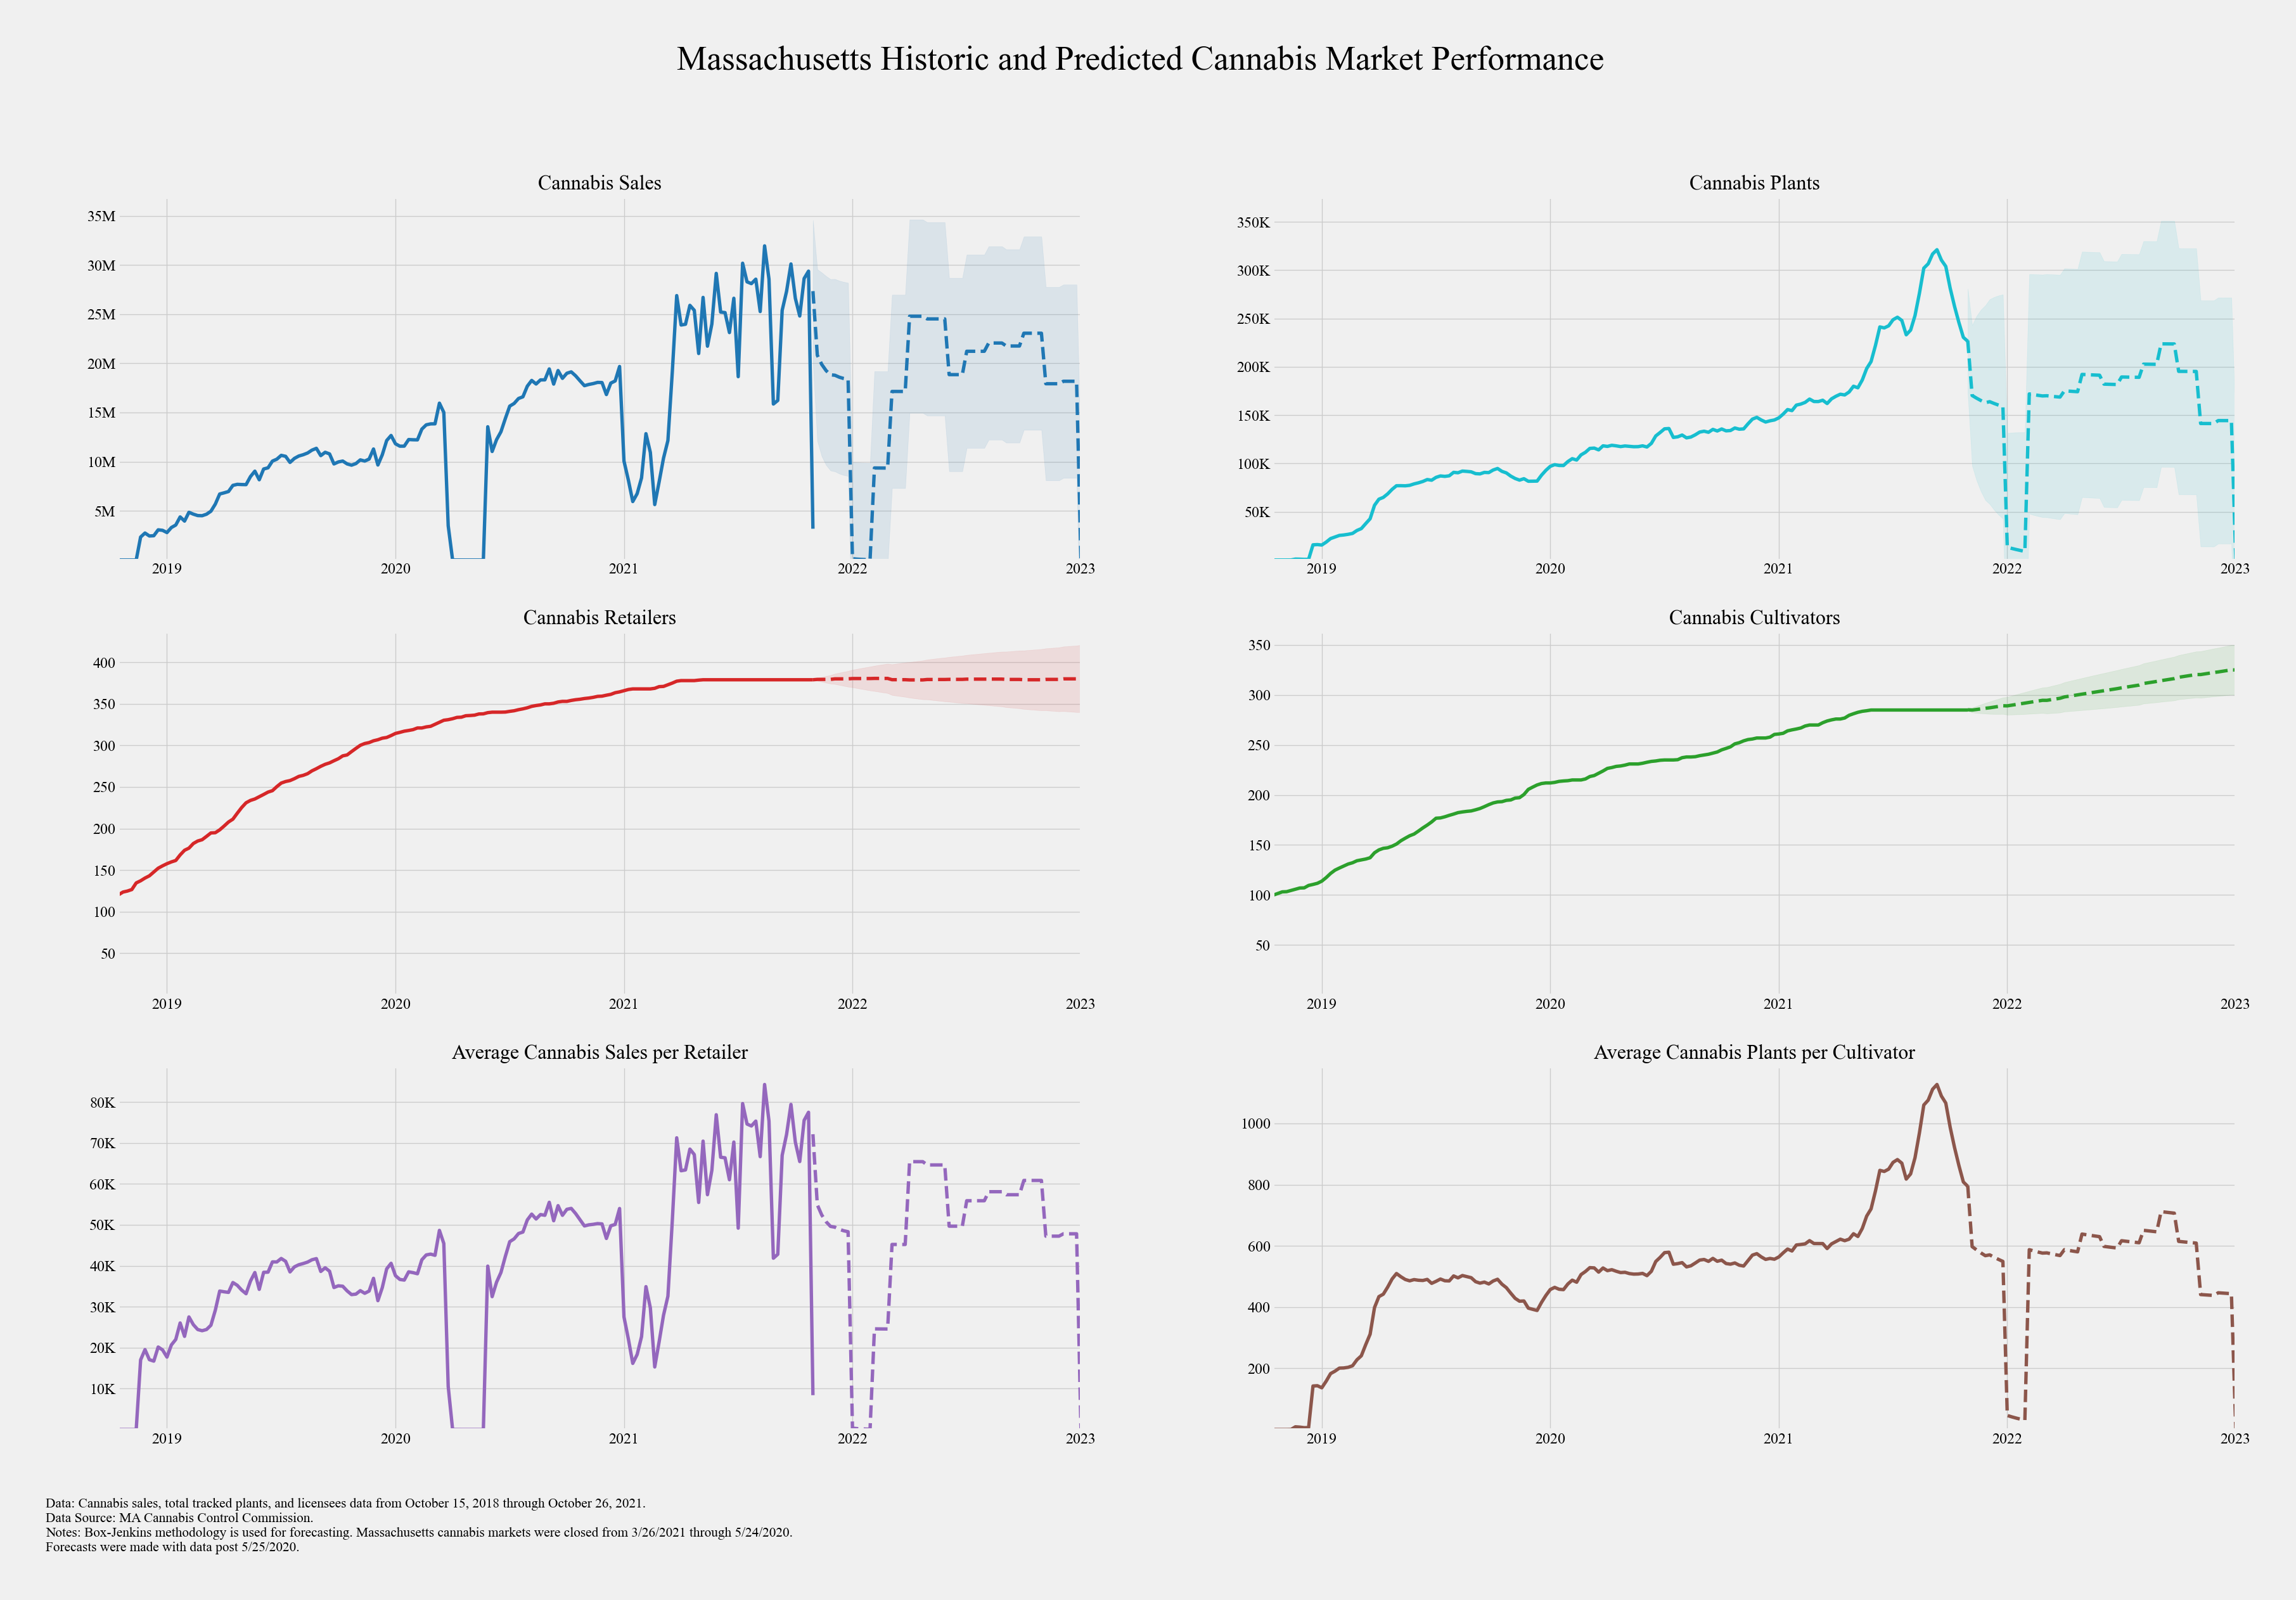
\includegraphics[width=\textwidth]{images/ma_market_forecast.png}
\end{center}

\end{frame}


\section{Economics}

\begin{frame}{}

{\large Structure, Conduct, and Performance}

\vspace{.75\baselineskip}

\begin{itemize}

\item Fathered by Edward S. Mason (1939).
\vspace{.75\baselineskip}
\item Seminal work by Joe Bain and George Stigler.
\vspace{.75\baselineskip}
\item Consequences: Antitrust policy.
\vspace{.75\baselineskip}
\item Criticisms: Chicago School (efficiencies and poor measurements).

\end{itemize}

\end{frame}

\begin{frame}{}

{\large Collusion}

\vspace{.75\baselineskip}

\begin{itemize}

\item Argument: Increased market concentration lowers the cost of collusion. A lower cost of collusion increases collusion between firms has an adverse affect on society.
\vspace{.75\baselineskip}
\item Counter-argument: Efficient firms will naturally gain market share and increased concentration may not necessarily lead to collusion. Thus, curtailing concentration could curtail efficiencies. 

\end{itemize}

\end{frame}


\begin{frame}{}

{\large Regulatory Capture}

\vspace{.75\baselineskip}

\begin{itemize}
\item Pioneering work by George Stigler.
\vspace{.75\baselineskip}
\item Argument: Regulatory agencies get ``captured'' by large producers to regulate at their behest and use regulation to prevent competition. {\tiny George J. Stigler Biography by David R. Henderson on Econlib.org}
\end{itemize}

\end{frame}


\section{Empirics}


\begin{frame}{}

``The questions concerning what number of firms is too large to permit collusion, and what amount of output control is sufficient for price setting, are essentially empirical issues.''

\vspace{.75\baselineskip}

{\tiny Reevaluation of the Structure-Conduct-Performance Paradigm in Banking.\\
Douglas D. Evanoff and Diana L. Fortier}

\end{frame}


\begin{frame}{}

{\large Measurements}

\vspace{.75\baselineskip}

\begin{itemize}
\item Measures of profitability.
\vspace{.75\baselineskip}
\item Measures of concentration.
\vspace{.75\baselineskip}
\item Measures of barriers to entry.
\vspace{.75\baselineskip}
\item Total factor of productivity measure.
\end{itemize}

\end{frame}

\section{Cannabis Applications}

%------------------------------------------------------
% Rules of Forecasting
%------------------------------------------------------

\begin{frame}{}

{\Large The 10 Commandments of Forecasting}\vspace{\baselineskip}\\

\begin{enumerate}
\item Know what you are forecasting.
\item Understand the purpose of forecasting.
\item Acknowledge the cost of the forecast error.
\item Rationalize the forecast horizon.
\item Understand the choice of variables.
\item Rationalize the forecasting model used.
\item Know how to present the results.
\item Know how to decipher the forecast results.
\item Use recursive methods.
\item Understand that forecasting models evolve over time.
\end{enumerate}
\end{frame}

\begin{frame}{}
\begin{center}
\begin{minipage}{3.85in}
\begin{block}{Until next time}
Study some economics, make some forecasts, and next week we can check our forecasts.
\end{block}

\end{minipage}
\end{center}
%
%{\Large References}\vspace{\baselineskip}\\
%
%\begin{enumerate}
%\item Inter-Industry Studies of Structure and Performance by Richard Schmalensee. Working Paper #1874-87. April 1987.
%\end{enumerate}

\end{frame}

%------------------------------------------------------------------%
\end{document}
%------------------------------------------------------------------%
